%接線に関する参考資料
\documentclass{jsarticle} \usepackage[dvipdfmx]{graphics} \usepackage{amsmath} \usepackage{amssymb} \usepackage{cases} \usepackage{ascmac}
\usepackage{url}
\usepackage{docmute}
\newcommand{\pt}{$(x_1,y_1)$}
\newcommand{\ptt}{$(p,q)$}
\renewcommand\thefootnote{*\arabic{footnote}}
\topmargin -0.8in
\textheight 10in


\title{二次曲線の接線に関する参考資料}
\author{}
\date{}

\begin{document}
\maketitle
    この参考資料で扱うのは、ある二次曲線上の点から引かれるその二次曲線の方程式を求めるという問題である。
    接線を求めよという問題に対して毎回微分して、傾きを出し直線の式を求めるのでは面倒である。
    様々な二次曲線の接線の方程式を導出する中で、その規則性を見出したい。

    %接線に関する参考資料
%\documentclass{jsarticle} \usepackage{graphics} \usepackage{amsmath} \usepackage{amssymb} \usepackage{cases}
%\newcommand{\pt}{$(x_1,y_1)$}

%\begin{document}
    \section{放物線}
    \subsection{導出}
    以下の放物線の\pt における接線を求める。
    \begin{equation}
        \label{eq:1-1}
        y=ax^2+ bx +c \hspace{3mm} (a \ne 0)
    \end{equation}
    式(\ref{eq:1-1})の両辺を$x$で微分し、
    \[
    \frac{{\rm d}y}{{\rm d}x} = 2ax +b
    \]
    \pt においては
    \[
    \frac{{\rm d}y}{{\rm d}x} = 2ax_1 +b
    \]
    これで$y=(2ax_1 +b)x$という部分が出来上がり、これは原点を通る直線だがこれを\pt に平行移動すればよい。
    \begin{eqnarray}
        (y-y_1) &=& (2ax_1 +b)(x-x_1) \label{eq:1-2}\\
        \Leftrightarrow y &=& (2ax_1 +b)x-2ax_1^2 -bx_1+y_1 \label{eq:1-3}
    \end{eqnarray}
    式(\ref{eq:1-3})がゴールといえる。しかし、算出は面倒なので式(\ref{eq:1-2})を式変形し以下の形を与えたい。
    \begin{eqnarray*}
        \frac{y-y_1}{2} &=& ax_1 x -ax_1^2 + b \cdot \frac{x-x_1}{2}\\
        (x_1,y_1)の条件より \hspace{3mm} y_1 &=& ax_1^2 +bx_1 +c \hspace{3mm} これを足す\\
    \end{eqnarray*}
    \begin{equation}
        \frac{y+y_1}{2} = ax_1 x +b \cdot \frac{x+x_1}{2} +c
        \label{eq:1-4}
    \end{equation}
    この式(\ref{eq:1-4})を放物線の接線の方程式の最終形としたい。
    \subsection{説明}
    式(\ref{eq:1-1})と式(\ref{eq:1-4})を見比べると座標\pt を用いて以下の置き換えを行っている。
    \begin{enumerate}
        \item
        \[
        x,\hspace{3mm} y\rightarrow \frac{x+x_1}{2} ,  \hspace{3mm} \frac{y+y_1}{2}
        \]
        \item
        \[
        x^2, \hspace{3mm} y^2 \rightarrow x_1 x, \hspace{3mm} y_1 y
        \]
    \end{enumerate}
    単純な書き換えではあるが、放物線にしか使えない規則かもしれない。これについては他の二次曲線に対しても適応できる規則なのか確認が必要である。

    \subsection{運用}
    実際に式(\ref{eq:1-4})が放物線に対して有効なのかを確認する。
    \[
    y=\frac{1}{9} x^2 -\frac{2}{9}x+1
    \]
    この放物線の$(2,1)$における接線の方程式を求める。式(\ref{eq:1-4})より接線の方程式は
    \begin{eqnarray*}
        \frac{y+1}{2} &=&\frac{1}{9}\cdot 2x -\frac{2}{9} \cdot \frac{x+2}{2} +1\\
        \Leftrightarrow y&=& \frac{2}{9} x-\frac{5}{9}
    \end{eqnarray*}
    以下の図は作図の結果である。
    \begin{figure}[htbp]
        \begin{center}
            \resizebox{!}{5cm}{
            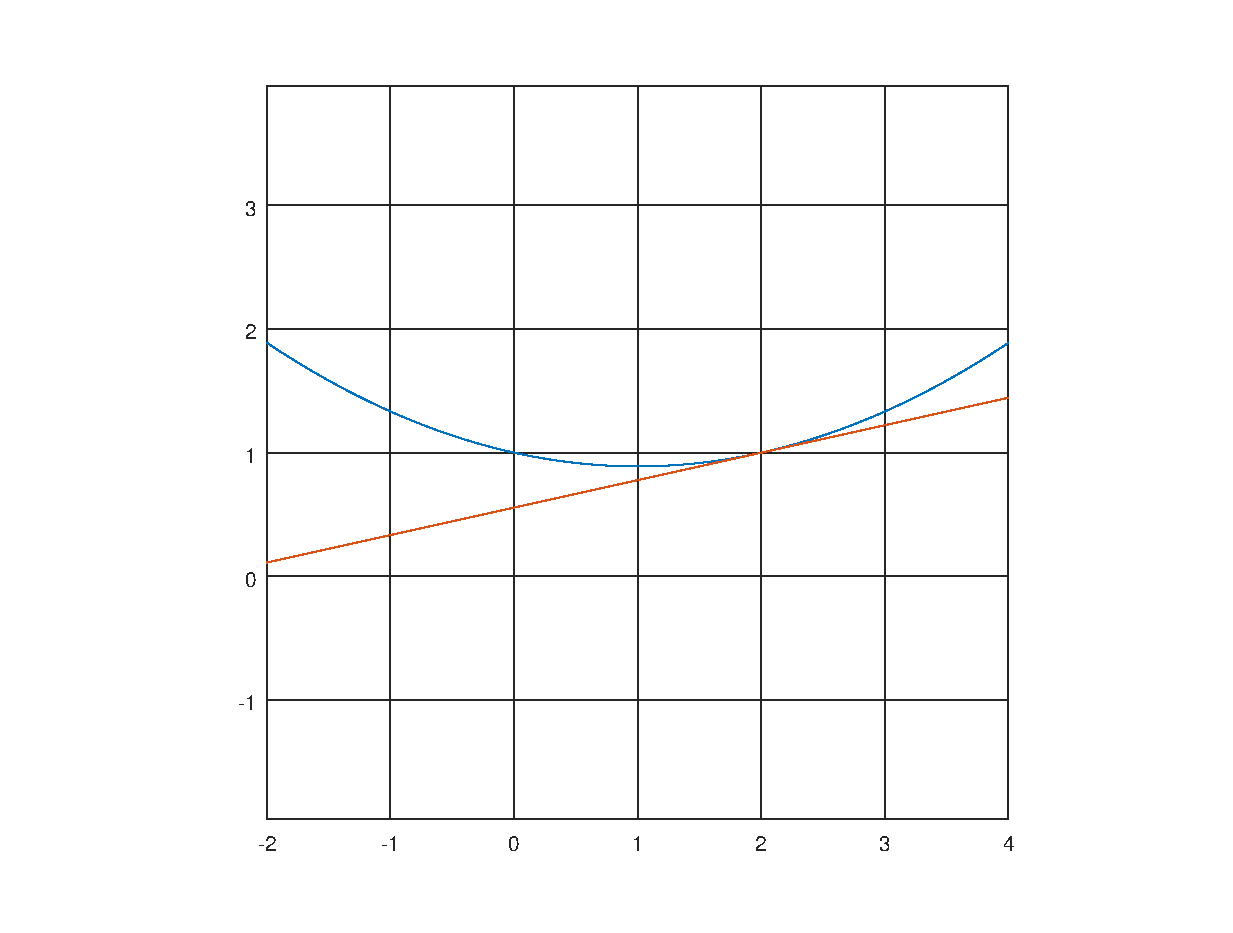
\includegraphics{1-1.eps}
            }
        \end{center}
        \caption{運用例}
        \label{fig:1-1}
    \end{figure}






%\end{document}

    %接線に関する参考資料
%\documentclass{jsarticle} \usepackage{graphics} \usepackage{amsmath} \usepackage{amssymb} \usepackage{cases}

%\newcommand{\pt}{$(x_1,y_1)$}
%\newcommand{\ptt}{$(p,q)$}

%\begin{document}
    \section{円}
    \subsection{導出}
    円の接線の方程式を導出するにはまず円の中心が原点にある時のものを考える。そのあと中心が原点にない場合を考えるが、この時は図形の平行移動を利用して簡単に求める。
    円の中心が原点にあるときの接線の導出には大きく2つの方法が考えられる。1つ目は円の接線と接点への半径は垂直であることから接線の傾きを決定する方法。2つ目は陰関数の微分を使って傾きを決定する方法。傾きの決定の方法が違うのみである。

    では早速、中心が原点にある半径$r$の円
    \[
    x^2 +y^2=r^2
    \]
    について円上の点\pt における接線を求める。傾きの求め方は2種類あるで分けて説明する。
    \begin{description}
        \item[円の接線の性質から傾きを求める] この方法をとる場合はいくつか場合分けをしなければならない。
        \begin{enumerate}
            \item $x_1 \neq 0$かつ$y_1 \neq 0$の時\\
            この時、原点から点\pt までの傾きは$\frac{y_1}{x_1}$なので接線の傾きは$-\frac{x_1}{y_1}$
            \item $x_1=0$の時\\
            この時は接点への半径が$y$軸と平行になるわけだから接線の傾きは$0$($x$軸と平行)となる。この結果は先の$x_1 \neq 0$かつ$y_1 \neq 0$の時の結果と合わせていいことがわかる。
            \item $y_1 = 0$の時\\
            この時は接点への半径が$x$軸と平行になるわけだから接線の傾きは$y$軸と平行\footnote{傾きが$y$軸と平行というのは厳密には傾きが定義できないということである。そのため多くの図形と方程式の問題で傾きが定義できない場合を特別視して場合分けする。}ということになる。
        \end{enumerate}
        以上から接線の傾きは$y_1 \neq 0$の時$-\frac{x_1}{y_1}$、$y_1 = 0$の時は傾きが定義できない、すなわち$y$軸と平行だということが分かった。
        \item[陰関数の微分から傾きを求める] 数I\hspace{-.1em}I\hspace{-.1em}Iの範囲であるため文系諸君は読み飛ばして構わない。\\
        \[
        x^2 +y^2=r^2
        \]
        の両辺を$x$で微分する。この方法でも$y_1 = 0$の場合を分けて考える。以下$y_1 \neq 0$である。
        \begin{eqnarray*}
            2x + 2y \cdot \frac{{\rm d}y}{{\rm d}x} &=& 0\\
            \Leftrightarrow \frac{{\rm d}y}{{\rm d}x} &=& -\frac{x}{y}
        \end{eqnarray*}
        よって\pt における接線の傾きは$-\frac{x_1}{y_1}$である。また$y_1 = 0$の時は先の方法と同様で接線の傾きは定義できない。
    \end{description}
    以上から接線の傾きを決定できた。ここから接線の方程式を求める。点\pt を通り傾き$-\frac{x_1}{y_1}$の直線の方程式は
    \begin{equation}
        y-y_1 = -\frac{x_1}{y_1} (x-x_1)
        \label{eq:2-1}
    \end{equation}
    確かに式(\ref{eq:2-1})で十分ではあるがここからさらに式変形を加えたい。
    \begin{eqnarray*}
        y-y_1 &=& -\frac{x_1}{y_1} (x-x_1)\\
        \Leftrightarrow y_1 y -y_1^2 &=& x_1^2 -x_1 x\\
        \Leftrightarrow x_1 x +y_1 y &=& x_1^2 +y_1^2\\
        &=& r^2
    \end{eqnarray*}
    以上の式変形から接線の方程式が
    \begin{equation}
        x_1 x +y_1 y= r^2
        \label{eq:2-2}
    \end{equation}
    であるとわかった。$y_1 = 0$の時は点$(x_1,0)$を通り$y$軸と平行なのだから接線の方程式は
    \[
    x=x_1
    \]
    となる。そもそもこの時の半径は$r=x_1$となるわけだから
    \[
    x=r
    \]
    となり、これは式(\ref{eq:2-2})によってあらわされる直線の1つといえる。

    このまま中心\ptt 、半径$r$の円のある円上の点\pt における接線の方程式を求める。まず円の方程式は
    \[
    (x-p)^2 +(y-q)^2=r^2
    \]
    である。このままだと式(\ref{eq:2-2})はうまく使えないため平行移動を使って円の中心と接点の両方を無理やり都合のいいところに移動する。すると円の方程式は
    \[
    x^2+y^2=r^2
    \]
    接点は$(x_1-p,y_1-q)$になる。こうなると式(\ref{eq:2-2})より接線の方程式は
    \[
    (x_1-p)x +(y_1-q)y=r^2
    \]
    となる。しかしこれは平行移動した後の結果であるため円の中心を\ptt に戻すようにもう一度平行移動しなければならない。ようやく答えは、
    \begin{equation}
        (x_1-p)(x-p) +(y_1-q)(y-q)=r^2
        \label{eq:2-3}
    \end{equation}
    このようになった。


    \subsection{確認}
    さて、放物線の方程式導出で明らかになった書き換えは覚えているだろうか。円の中心が原点にあるときの接線に関しては式(\ref{eq:2-2})から規則が成立しているのは明らかだが中心が原点にない場合を確認する。
    \[
    (x-p)^2 +(y-q)^2=r^2
    \]
    これを展開すると
    \[
    x^2-2px+y^2-2qy+p^2+q^2=r^2
    \]
    となる。この形を覚えてもらいたい。そして式(\ref{eq:2-3})を式変形する。
    \begin{eqnarray*}
        (x_1-p)(x-p) +(y_1-q)(y-q) &=& r^2\\
        \Leftrightarrow x_1 x -p(x +x_1) +p^2 +y_1 y -q(y+y_1) +q^2 &=& r^2\\
        \Leftrightarrow x_1 x -2p \cdot \frac{x +x_1}{2} +y_1 y -2q \cdot \frac{y+y_1}{2} +p^2 +q^2 &=& r^2
    \end{eqnarray*}
    これで規則の成立を確認できた。


%\end{document}




    %接線に関する参考資料
%\documentclass{jsarticle} \usepackage{graphics} \usepackage{amsmath} \usepackage{amssymb} \usepackage{cases} \usepackage{ascmac}

%\newcommand{\pt}{$(x_1,y_1)$}


%\begin{document}
    \section{まとめ}
    これまでの話から、ある二次曲線の接線を求めるときその二次曲線上の点を\pt とすると以下の書き換えで接線の方程式が導出できるとわかった。

    \begin{shadebox}
        \begin{itemize}
            \item $x,y$が1次の項
            \[
            x,\hspace{3mm} y\rightarrow \frac{x+x_1}{2} ,  \hspace{3mm} \frac{y+y_1}{2}
            \]
            \item $x,y$が2次の項
            \[
            x^2, \hspace{3mm} y^2 \rightarrow x_1 x, \hspace{3mm} y_1 y
            \]
        \end{itemize}
    \end{shadebox}
    この置き換えを行う条件は二次曲線の方程式が完全に展開されていることであることを注意として述べておく。便利な計算の方法として覚えてもらいたい。



%\end{document}

    \newpage
    \documentclass[dvipdfmx]{jsarticle}
\usepackage{graphics}
\usepackage{amsmath}
\usepackage{amssymb}
\usepackage{amsthm}
\usepackage{mathtools}
\usepackage{ascmac}
\usepackage{bm}
\usepackage{url}
\usepackage{txfonts}
\usepackage{color}
\usepackage{tikz}
% \usepackage{docmute}    %パッケージのダウンロードが必要
\usepackage{tikz}
\usetikzlibrary{calc}
\usetikzlibrary{intersections}

\begin{document}
    \section*{最後に}
    本資料は以下のURLのサイトに掲載されているものです.

    {\centering \url{https://blkdenden.firebaseapp.com/lib.html}\\}

    転載などはしないでください.

    また,誤植などは順次訂正しますが,不明な点は掲載サイトのコンタクト欄からメールを送信,または以下のメールアドレスに問い合わせてください.

    {\centering \url{s.kondo11235813@gmail.com}\\}

    % \section*{参考文献}
    % \begin{itemize}
    %     \item 『高等学校 数学B』,数研出版(2017)
    % \end{itemize}




\end{document}


\end{document}
